\documentclass[a4paper,fleqn,12pt,twoside]{article}

\parindent=0pt
\parskip=2pt

\usepackage{amsfonts}	%% for \mathbb
\usepackage{bm}		%% bold math symbols
\usepackage{tikz}
\usepackage{placeins}
\usepackage{hyperref}

\newcommand\todo{\bigskip\fbox{TODO}\bigskip}

\newcommand{\hb}[2]{paragraph #2 on page #1 of the Handbook}
\newcommand{\hbm}[2]{{\marginpar{\scriptsize \sl Handbook #1, #2}}}

\newcommand\Arg{{\rm Arg}}
\newcommand\Log{{\rm Log}}
\newcommand\RE{{\rm Re}}
\newcommand\IM{{\rm Im}}

\newcommand\Complex{\mathbb{C}}
\newcommand\Integer{\mathbb{Z}}
\newcommand\Real{\mathbb{R}}

\title{Solutions to the M337/B 2013 exam paper}
\author{Edited by: Fred Youhanaie}
\date{12 June, 2013}

\begin{document}
\maketitle

\pagestyle{myheadings}
\markboth{M337/B 2013}{M337/B 2013}	% two sided
%%\markright{M337/B 2013}		% one sided

\section*{Copyright}

This work is licensed under a Creative Commons
Attribution-NonCommercial-ShareAlike 3.0 Unported License.

\newcommand\cclink{http://creativecommons.org/licenses/by-nc-sa/3.0/}
See the \href{\cclink}{by-nc-sa page}\footnote{\cclink} for details.

\section*{Solutions to Part I}
\subsection*{Solution 1}

\begin{itemize}
\item[(a)]

\begin{eqnarray*}
\exp(3+\frac{1}{4}\pi i)
	&=& e^3 \left( \cos \left(\frac{\pi}{4}\right) + i \sin \left(\frac{\pi}{4}\right) \right) \\
	&=& \frac{e^3}{\sqrt{2}} + i\frac{e^3}{\sqrt{2}}
\end{eqnarray*}

\item[(b)]
Let
\[ w^3 = -8 = 8( \cos\pi + i\sin\pi ) \]
then, \hbm{A1}{3.3}
\begin{eqnarray*}
w	&=& 8^\frac{1}{3} ( \cos ( \pi/3 ) + i \sin ( \pi/3 ) ) \\
	&=& 2 \left( \frac{1}{2} + i \frac{\sqrt{3}}{2} \right) \\
	&=& 1 + \sqrt{3}\,i
\end{eqnarray*}

\item[(c)]
Using the Principal $\alpha$th power:\hbm{A2}{5.3}
\begin{eqnarray*}
i^{1-2i}
	&=& \exp( (1-2i) \Log(i)) \\
	&=& \exp( (1-2i) (\log_e|i| + i\Arg(i) ) ) \\
	&=& \exp( i\pi/2 - 2i^2\pi/2 ) \\
	&=& \exp( \pi + i\pi/2 ) \\
	&=& e^\pi e^{i\pi/2} \\
	&=& e^\pi ( \cos(\pi/2) + i\sin(\pi/2) ) \\
	&=& ie^\pi
\end{eqnarray*}

\item[(d)]
Using the trigonometric functions\hbm{A2}{4.4}
\begin{eqnarray*}
\cos(i\log_e 2)
	&=& \frac{1}{2} \left( \exp(i^2\log_e 2) + \exp(-i^2\log_e 2) \right) \\
	&=& \frac{1}{2} \left( \exp(-\log_e 2) + \exp(\log_e 2) \right) \\
	&=& \frac{1}{2} \left( 1/2 + 2 \right) \\
	&=& \frac{5}{4}
\end{eqnarray*}

\end{itemize}


\newpage
\subsection*{Solution 2}

\begin{itemize}
\item[(a)][FY,LK]

Below are the sketches of the four sets:

%
%	Sketches for Q2

%
%	Set A
%
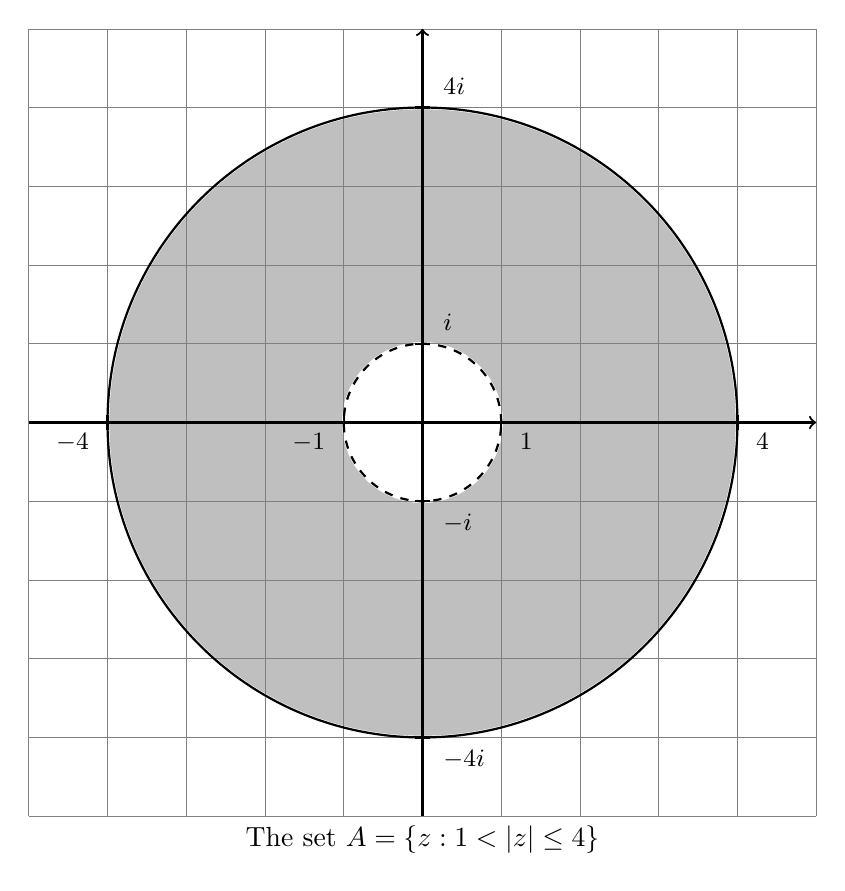
\begin{tikzpicture}
	% shading - must be drawn before the rest!
	\filldraw[even odd rule,color=lightgray] (0,0) circle(3.97) (0,0) circle(1.03);
	% grid for draft only
	\draw [help lines] (-5,-5) grid (5,5);
	% legend
	\draw (0,-5) node[below] {The set $A=\{z:1<|z|\le4\}$};
	% the X-axis
	\draw[->,thick] (-5,0)--(5,0);
	\draw[thick] (-4,-0.1) -- (-4,0.1) node[below left=3pt] {\small $-4$};
	\draw[thick] (-1,-0.1) -- (-1,0.1) node[below left=3pt] {\small $-1$};
	\draw[thick] (1,-0.1) -- (1,0.1) node[below right=3pt] {\small $1$};
	\draw[thick] (4,-0.1) -- (4,0.1) node[below right=3pt] {\small $4$};
	% the Y-axis
	\draw[->,thick] (0,-5)--(0,5);
	\draw[thick] (-0.1,-4) -- (0.1,-4) node[below right=1pt] {\small $-4i$};
	\draw[thick] (-0.1,-1) -- (0.1,-1) node[below right=1pt] {\small $-i$};
	\draw[thick] (-0.1,1) -- (0.1,1) node[above right=1pt] {\small $i$};
	\draw[thick] (-0.1,4) -- (0.1,4) node[above right=1pt] {\small $4i$};
	% inner circle border
	\draw[thick,style=dashed] (0,0) circle (1);
	% outer circle border
	\draw[thick] (0,0) circle (4);
\end{tikzpicture}

\bigskip

%
%	Set B
%
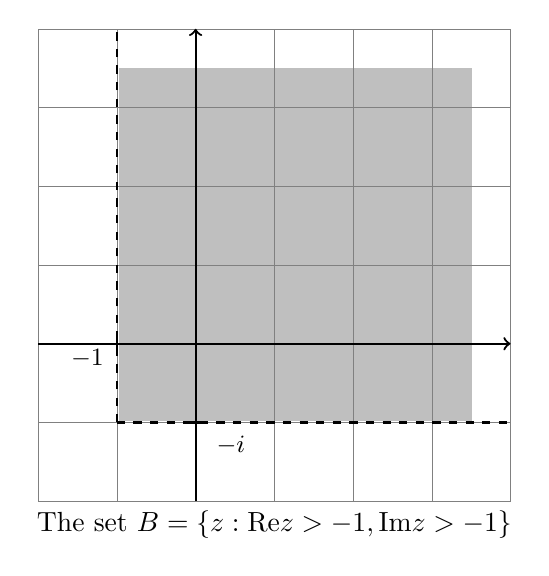
\begin{tikzpicture}
	% shading - must be drawn before the rest!
	\filldraw[color=lightgray] (-0.97,-0.97) -- (3.5,-0.97) -- (3.5,3.5) -- (-0.97,3.5) -- cycle;
	% grid for draft only
	\draw [help lines] (-2,-2) grid (4,4);
	% legend
	\draw (1,-2) node[below] {The set $B=\{z:\RE z>-1,\IM z>-1\}$};
	% the Y-axis
	\draw[->,thick] (0,-2)--(0,4);
	% the X-axis
	\draw[->,thick] (-2,0)--(4,0);
	\draw[thick] (-1,-0.1) -- (-1,0.1) node[below left=1pt] {\small $-1$};
	\draw[thick] (-0.1,-1) -- (0.1,-1) node[below right=1pt] {\small $-i$};
	% the two borders
	\draw[style=dashed,thick] (-1,-1) -- (4,-1);
	\draw[style=dashed,thick] (-1,-1) -- (-1,4);
\end{tikzpicture}

\bigskip

%
%	Set C
%
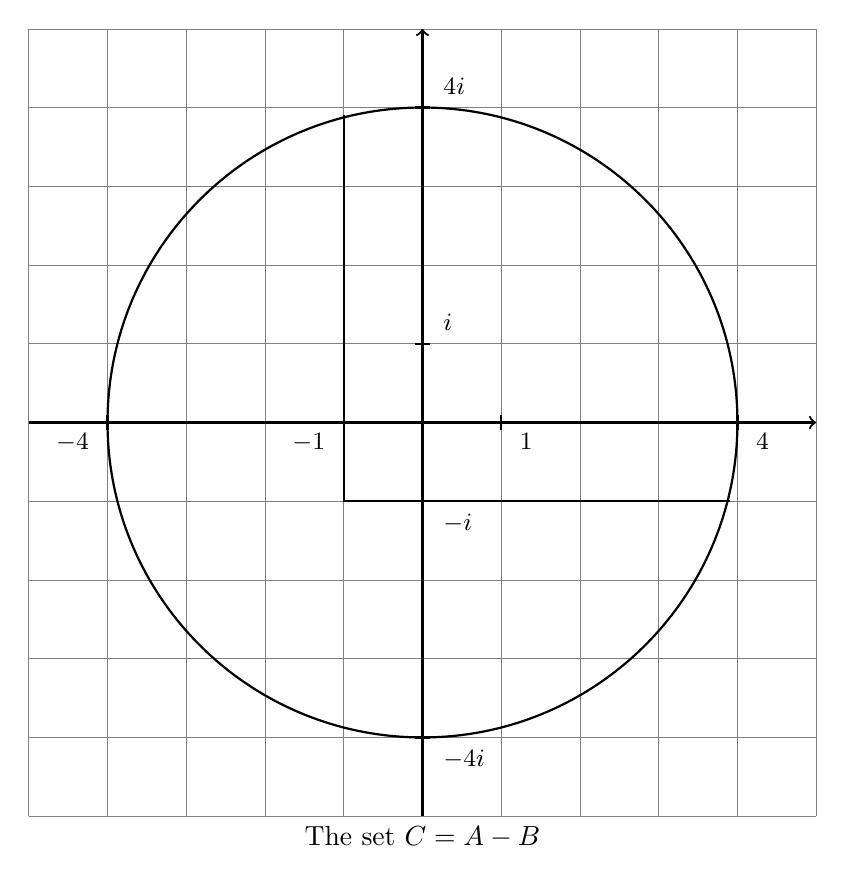
\begin{tikzpicture}
	% shading - must be drawn before the rest!
	%%\filldraw[even odd rule,color=lightgray] (0,0) circle(3.97) (0,0) circle(1.03);
	% grid for draft only
	\draw [help lines] (-5,-5) grid (5,5);
	% legend
	\draw (0,-5) node[below] {The set $C=A-B$};
	% the X-axis
	\draw[->,thick] (-5,0)--(5,0);
	\draw[thick] (-4,-0.1) -- (-4,0.1) node[below left=3pt] {\small $-4$};
	\draw[thick] (-1,-0.1) -- (-1,0.1) node[below left=3pt] {\small $-1$};
	\draw[thick] (1,-0.1) -- (1,0.1) node[below right=3pt] {\small $1$};
	\draw[thick] (4,-0.1) -- (4,0.1) node[below right=3pt] {\small $4$};
	% the Y-axis
	\draw[->,thick] (0,-5)--(0,5);
	\draw[thick] (-0.1,-4) -- (0.1,-4) node[below right=1pt] {\small $-4i$};
	\draw[thick] (-0.1,-1) -- (0.1,-1) node[below right=1pt] {\small $-i$};
	\draw[thick] (-0.1,1) -- (0.1,1) node[above right=1pt] {\small $i$};
	\draw[thick] (-0.1,4) -- (0.1,4) node[above right=1pt] {\small $4i$};
	% inner border
	\draw[thick] (-1,3.9) -- (-1,-1) -- (3.9,-1);
	% outer circle/arc
	\draw[thick] (0,0) circle (4);
\end{tikzpicture}

\bigskip

%
%	Set D
%
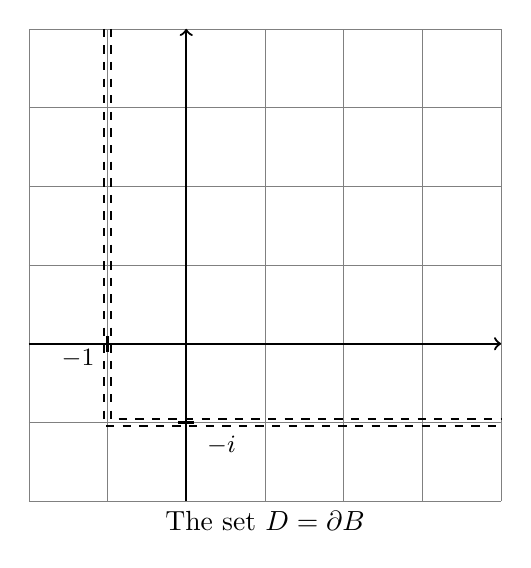
\begin{tikzpicture}
	% grid for draft only
	\draw [help lines] (-2,-2) grid (4,4);
	% legend
	\draw (1,-2) node[below] {The set $D=\partial B$};
	% the Y-axis
	\draw[->,thick] (0,-2)--(0,4);
	% the X-axis
	\draw[->,thick] (-2,0)--(4,0);
	\draw[thick] (-1,-0.1) -- (-1,0.1) node[below left=1pt] {\small $-1$};
	\draw[thick] (-0.1,-1) -- (0.1,-1) node[below right=1pt] {\small $-i$};
	% the empty border!
	% - outer side of the L
	\draw[thick,style=dashed] (-1.04,4) -- (-1.04,-1.04) -- (4,-1.04);
	% - inner side of the L
	\draw[thick,style=dashed] (-0.96,4) -- (-0.96,-0.96) -- (4,-0.96);
\end{tikzpicture}



\item[(b)]
\begin{itemize}
\item[(i)][FY,LK]

\begin{itemize}
\item[$A$] is not a region, not open
\item[$B$] is a region
\item[$C$] is not a region, not open
\item[$D$] is not a region, not open
\end{itemize}

\item[(ii)]

\begin{itemize}
\item[$A$] is not compact, not closed
\item[$B$] is not compact, not closed
\item[$C$] is not compact, not closed
\item[$D$] is not compact, not bounded
\end{itemize}

\end{itemize}

\end{itemize}


\newpage
\subsection*{Solution 3}

\begin{itemize}
\item[(a)]
By definition \hbm{A2}{2.3}
\[ \Gamma: \gamma(t) = 2(\cos(t) + i\sin(t)) = 2e^{it},\;\; (t\in[0,2\pi]) \]

\item[(b)]
We use the polar form from above,
\begin{eqnarray*}
\overline{\gamma(t)}
	&=& 2e^{-it}\\
\\
\gamma'(t)
	&=& 2ie^{it}
\end{eqnarray*}
So,\hbm{B1}{2.1}
\begin{eqnarray*}
\int_\Gamma \overline{z}\,dz
	&=& \int_0^{2\pi} \left( 2e^{-it} 2ie^{it} \right) \, dt \\
	&=& \int_0^{2\pi} 4i\,dt \\
	&=& \left[ 4it \right]_0^{2\pi} \\
	&=& 8\pi i
\end{eqnarray*}

\item[(c)][FY,LK]
Let
\[ f(z) = \frac{ 2\sin z }{ \overline{z}^2+1 } \]
then, $f$ is continuous on $\Gamma$ by combination rules, where $\Gamma$
has length $L=4\pi$


So, using the triangle inequality\hbm{A1}{5.2(a)}
\begin{eqnarray*}
|2\sin z|
	&=& \left| 2\frac{1}{2i} \left( e^{iz} - e^{-iz} \right) \right| \\
	&=& \left| -i \left( e^{iz} - e^{-iz} \right) \right| \\
	&\le& \left| e^{iz} \right| + \left| e^{-iz} \right| \\
	&=& e^{\RE\,z} + e^{-\RE\,z} \\
	&<& 2e^2
\end{eqnarray*}
%%
And, using the backward triangle inequality\hbm{A1}{5.2(b)}
\begin{eqnarray*}
\left| \overline{z}^2+1 \right|
	&\ge& \left| |z|^2 - |1| \right| \\
	&=& |4-1| \\
	&=& 3
\end{eqnarray*}
%%
So,
\begin{eqnarray*}
|f(z)|	&=& \left| \frac{ 2\sin z }{ \overline{z}^2+1 } \right| \\
	&=& \frac{ |2\sin z| }{ \left| \overline{z}^2+1 \right| } \\
	&\le& \frac{2e^2}{3} \\
	&=& M
\end{eqnarray*}
%%
then by the Estimation Theorem.\hbm{B1}{4.3}
\[
\left| \int_\Gamma \frac{ 2\sin z }{ \overline{z}^2+1 }\,dz \right|
\le ML = \frac{2e^2}{3} 4\pi = \frac{8\pi e^2}{3} 
\]

\end{itemize}


\newpage
\subsection*{Solution 4}

\begin{itemize}
\item[(a)]

Let $R=\{ z: |z|<2 \}$, and $f(z)=\frac{\Log(2-z)}{z^2+4}$, then
\begin{enumerate}
\item $R$ is a simply-connected region
\item $f$ is analytic on $R$
\item $C$ is a closed contour in $R$
\end{enumerate}
Hence, by Cauchy's Theorem\hbm{B2}{1.4}
\[
\int_C \frac{\Log(2-z)}{z^2+4}\,dz = 0
\]

\item[(b)]

Let $R=\{ z: |z|<2 \}$, and $f(z)=\frac{\Log(2-z)}{z-2}$, then
\begin{enumerate}
\item $R$ is a simply-connected region
\item $f$ is analytic on $R$
\item $C$ is a simple-closed contour in $R$
\item $z=0$ is inside $C$
\end{enumerate}
Hence, by Cauchy's Integral Formula \hbm{B2}{2.1}
\begin{eqnarray*}
f(0)	&=& \frac{1}{2\pi i} \int_C \frac{f(z)}{z}\, dz \\
	&=& \frac{1}{2\pi i} \int_C \frac{\Log(2-z)/(z-2)}{z}\, dz \\
\end{eqnarray*}
where,
\[ f(0) = \Log(2)/(-2) = -\log_e 2/2 \]

\[
\int_C \frac{\Log(2-z)}{z(z-2)}\,dz = -\frac{\log_e 2}{2}\times2\pi i = -\pi\log_e 2\,i
\]

\item[(c)][FY,JK]

Let $R=\{ z: |z|<2 \}$, and $f(z)=\Log(2-z)$, then
\begin{enumerate}
\item $R$ is a simply-connected region
\item $f$ is analytic on $R$
\item $C$ is a simple-closed contour in $R$
\item $z=0$ is inside $C$
\item $f$ is differentiable at $z=0$
\end{enumerate}
Hence, by Cauchy's 2nd Derivative Formula\hbm{B2}{3.1}
\begin{eqnarray*}
f^{(2)}(0)
	&=& \frac{2!}{2\pi i} \int_C \frac{ f(z) }{ z^3 }\, dz \\
	&=& \frac{1}{\pi i} \int_C \frac{ \Log(2-z) }{ z^3 }\, dz
\end{eqnarray*}
where,
\begin{eqnarray*}
f'(z)	&=& -\frac{1}{2-z} \\
f^{(2)}(z)
	&=& -\frac{1}{(2-z)^2}
\end{eqnarray*}
So,
\[
\int_C \frac{ \Log(2-z) }{ z^3 }\,dz = f^{(2)}(0)\pi i = -\frac{\pi i}{4}
\]

\end{itemize}


\newpage
\subsection*{Solution 5}

\begin{itemize}
\item[(a)]

$f$ has three simple poles at 0, 1/5 and 5. We shall use the cover-up
rule to obtain the residues.\hbm{C1}{1.3}
%%
\begin{eqnarray*}
\Res(f, 0)
	&=& \frac{ z^2+1 }{ (5z-1)(z-5) } \\
	&=& \frac{1}{(-1)(-5)} \\
	&=& \frac{1}{5} \\
\\
\Res(f, 1/5)
	&=& \frac{ z^2+1 }{ 5z(z-5) } \\
	&=& \frac{ (1/5)^2+1 }{ 5(1/5)(1/5-5) } \\
	&=& \frac{ 26/25 }{ -24/5 } \\
	&=& -\frac{13}{60} \\
\\
\Res(f, 5)
	&=& \frac{ z^2+1 }{ z(5z-1) } \\
	&=& \frac{ 25+1 }{ 5(25-1) } \\
	&=& \frac{13}{60}
\end{eqnarray*}

\item[(b)]

We shall use the strategy for evaluating
$\int_0^{2\pi}\Phi(\cos t, \sin t)\,dt$.
\hbm{C1}{2.2}

After replacements, we have, for $C=\{z:|z|=1\}$
\begin{eqnarray*}
\int_0^{2\pi} \frac{ \cos t }{ 13-5\cos t }\,dt
	&=& \int_C \frac{ \frac{1}{2}(z+1/z) }{ 13-\frac{5}{2}(z+1/z) } \times \frac{1}{iz}\,dz \\
	&=& \int_C \frac{ z^2+1 }{ 26z-5z^2-5 } \times \frac{1}{iz}\,dz \\
	&=& i \int_C \frac{ z^2+1 }{ z(5z^2-26z+5) }\,dz \\
	&=& i \int_C \frac{ z^2+1 }{ z(5z-1)(z-5) }\,dz \\
	&=& i \int_C f(z)\,dz
\end{eqnarray*}
%%
Now, $f(z)$ is analytic on $\Complex$, a simply-connected region,
exceptn for the three singularities. The unit circle $C$ is a
simple-closed contour in $\Complex$, which does not pass through $f$'s
singularities, then by Cauchy's Residue Theorem\hbm{C1}{2.1}
\begin{eqnarray*}
\int_C f(z)\,dz
	&=& 2\pi i\left(\Res(f,0)+\Res(f,1/5)\right) \\
	&=& 2\pi i\left(\frac{1}{5}-\frac{13}{60}\right) \\
	&=& -\frac{\pi i}{30}
\end{eqnarray*}
%%
Hence,
\[
\int_0^{2\pi} \frac{ \cos t }{ 13-5\cos t }\,dt
	= i \int_C f(z)\,dz
	= i \left( -\frac{\pi i}{30} \right)
	= \frac{\pi}{30}
\]

\end{itemize}


\newpage
\subsection*{Solution 6}

\begin{itemize}
\item[(a)]
\todo
\item[(b)]
\todo
\end{itemize}


\newpage
\subsection*{Solution 7}

\begin{itemize}
\item[(a)]
\todo
\item[(b)]
\todo
\item[(c)]
\todo
\end{itemize}


\newpage
\subsection*{Solution 8}

\begin{itemize}
\item[(a)]

The iteration sequence
\[
z_{n+1} = 15z_n^2 + 3z_n + \frac{1}{16}
\]
is conjugate to the iteration sequence\hbm{D3}{2.1}
\[
w_{n+1} = w_n+d
\]
where
\[
d = \frac{15}{16} + \frac{3}{2} - \frac{9}{4} = \frac{15+24-36}{16} = \frac{3}{16}
\]
so, $w_{n+1} = w_n+\frac{3}{16}$.
The conjugating function is
\[
h(z) = 15z+\frac{1}{2}\times3 = 15z+\frac{3}{2}
\]
So, $w_0 = h(z_0) = h(0) = 0+\frac{3}{2} = \frac{3}{2}$

\item[(b)][FY,LK]

$P_{\frac{3}{16}}$ has fixed points at $z$, where $z^2+\frac{3}{16}=z$,
these are the solutions to the equation
\[
z^2-z+\frac{3}{16} = 0
\]
So
\[
z = \frac{ 1 \pm \sqrt{1 - 12/16} }{ 2 } = \frac{ 1 \pm \sqrt{1/4} }{ 2 } = \frac{1}{2}\pm\frac{1}{4}
\]
Hence, the fixed points of $P_{\frac{3}{16}}$ are $\frac{3}{4}$ and $\frac{1}{4}$.

Now, $P'_{\frac{3}{16}}(z) = 2z$, so
\[ \left|P'_{\frac{3}{16}}\left(\frac{3}{4}\right)\right| = \frac{6}{4} = \frac{3}{2} > 1 \]
and
\[ \left|P'_{\frac{3}{16}}\left(\frac{1}{4}\right)\right| = \frac{2}{4} = \frac{1}{2} < 1 \]
Hence, $\frac{1}{4}$ is an attracting fixed point and $\frac{3}{4}$
is a repelling one.\hbm{D3}{1.5}

\item[(c)]

Let $c=-\frac{3}{2}+i$, then it appears from the diagram that $c$ is
outside the Mandelbrot set.\hbm{D3}{4.3}

Using the specification for $M$\hbm{D3}{4.5}
\[
|P_c(0)| = |-3/2+i| = \sqrt{9/4+1} = \sqrt{13/4} < 2
\]
We go for the next iteration:
\begin{eqnarray*}
|P_c^{(2)}(0)|
	&=& |(-3/2+i)^2-3/2+i| \\
	&=& |9/4-1-3i-3/2+i| \\
	&=& |-1/4-2i| \\
	&=& \sqrt{1/16+4} \\
	&=& \sqrt{65/4} \\
	&\simeq& 4.0 > 2
\end{eqnarray*}
Hence, $c$ lies outside the Mandelbrot set, $c\not\in M$.

\end{itemize}


\newpage

\section*{Solutions to Part II}
\subsection*{Solution 9}

\begin{itemize}
\item[(a)]

\begin{itemize}
\item[(i)]
\todo
\item[(ii)]
\todo
\item[(iii)]
\todo
\end{itemize}

\item[(b)]

\begin{itemize}
\item[(i)]
\todo
\item[(ii)]
\todo
\item[(iii)]
\todo
\item[(iv)]
\todo
\item[(v)]
\todo
\item[(vi)]
\todo
\end{itemize}

\end{itemize}


\newpage
\subsection*{Solution 10}

\begin{itemize}
\item[(a)]

\begin{itemize}

\item[(i)]

The function $f(z)$ has two simple poles at $z=1$ and $z=5$.

\item[(ii)]

A sketch of the annulus is shown below:

%
%	Sketches for Q10(a)(i)

%
%	The annulus {z: 1 < |z-2| < 3}
%
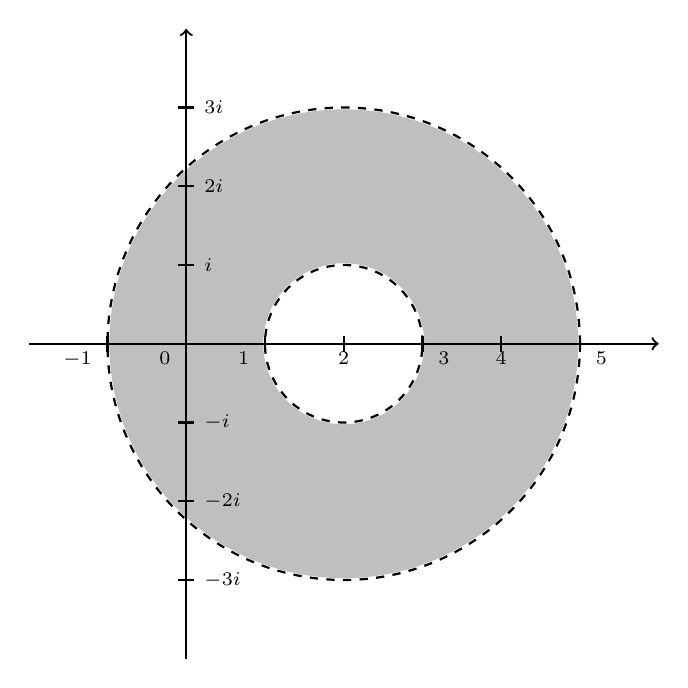
\begin{tikzpicture}
	% shading - must be drawn before the rest!
	\filldraw[even odd rule,color=lightgray] (2,0) circle(2.97) (2,0) circle(1.03);
	% grid for draft only
	%%\draw [help lines] (-2,-4) grid (6,4);
	% the X-axis
	\draw[->,thick] (-2,0)--(6,0);
	\foreach \x in {-1, 0, 1} {
		\draw[thick] (\x,-0.1) -- (\x,0.1) node[below left=2pt] {\scriptsize $\x$};
	}
	\foreach \x in {2, 4} {
		\draw[thick] (\x,-0.1) -- (\x,0.1) node[below=2pt] {\scriptsize $\x$};
	}
	\foreach \x in {3, 5} {
		\draw[thick] (\x,-0.1) -- (\x,0.1) node[below right=2pt] {\scriptsize $\x$};
	}
	% the Y-axis
	\draw[->,thick] (0,-4)--(0,4);
	\foreach \y in {2, 3} {
		\draw[thick] (-0.1,-\y) -- ( 0.1,-\y) node[right] {\scriptsize $-\y i$};
		\draw[thick] (-0.1, \y) -- ( 0.1, \y) node[right] {\scriptsize $ \y i$};
	}
	\draw[thick] (-0.1,-1) -- (0.1,-1) node[right] {\scriptsize $-i$};
	\draw[thick] (-0.1, 1) -- (0.1, 1) node[right] {\scriptsize $ i$};
	% inner circle border
	\draw[thick,style=dashed] (2,0) circle (1);
	% outer circle border
	\draw[thick,style=dashed] (2,0) circle (3);
\end{tikzpicture}



\todo
\end{itemize}

\item[(b)]

\begin{itemize}
\item[(i)]
\todo
\item[(ii)]
\todo
\end{itemize}

\end{itemize}


\newpage
\subsection*{Solution 11}

\begin{itemize}
\item[(a)]

We shall use the Cover-up rule\hbm{C1}{1.3} to obtain the residues at
the three simple poles at $0$, $\frac{3}{4}i$ and $-\frac{3}{4}i$:
\[
f(z)	= \frac{ \pi\cot(\pi z) }{ 16z^2+9) }
	= \frac{ \pi \cos(\pi z) }{ (4z-3i)(4z+3i)\sin(\pi z) }
\]
Hence,
\begin{eqnarray*}
\Res(f,0)
	&=& \frac{ \pi \cos(\pi z) }{ (4z-3i)(4z+3i) } \\
	&=& \frac{ \pi }{ (-3i)(3i) } \\
	&=& \frac{ \pi }{ 9 } \\
\\
\Res\left(f,\frac{3}{4}i\right)
	&=& \frac{ \pi \cos(\pi z) }{ 4(4z+3i)\sin(\pi z) } \\
	&=& \frac{ \pi/\sqrt{2} }{ 4(3i+3i)/(-\sqrt{2}) } \\
	&=& -\frac{ \pi }{ 24i } \\
	&=& \frac{\pi}{24}i \\
\\
\Res\left(f,-\frac{3}{4}i\right)
	&=& \frac{ \pi \cos(\pi z) }{ 4(4z-3i)\sin(\pi z) } \\
	&=& \frac{ -\pi/\sqrt{2} }{ 4(-3i-3i)/(-\sqrt{2}) } \\
	&=& \frac{ \pi }{ 24i } \\
	&=& -\frac{\pi}{24}i
\end{eqnarray*}

\item[(b)]
\todo
\item[(c)]
\todo
\end{itemize}


\newpage
\subsection*{Solution 12}

\begin{itemize}
\item[(a)]
\todo
\item[(b)]

\begin{itemize}
\item[(i)]
\todo
\item[(ii)]
\todo
\item[(iii)]
\todo
\item[(iv)]
\todo
\end{itemize}

\end{itemize}



\end{document}

